%%%%%%%
% Ch2 %
%%%%%%%

\chapter{Redresseur à diodes}
	
	Ils sont simples, bon marché et ne nécessitent aucun réglage, délivrent une tension continue essentiellement constante sur base d'une tension alternative. Il existe deux catégories de charges à alimenter, celles pour lesquelles il faut délivré une tension continue lisse et celle pour lesquelles il faut limiter la déformation du signal. Les équipements électroniques appartiennent à la 1ère catégorie, c'est pourquoi on retrouve un condensateur connecté entre les bornes de sortie qui permet de lisser le signal redressé. Les machines à courant continu, charges dites $RLE$, appartiennent à la 2è catégorie, nécessite un redresseur à thyristors (\textbf{commandable}) puisque celui à diode est \textbf{non-commandable}. La liste des symbole utilisé est repris ci-dessous.
	
	\begin{center}
	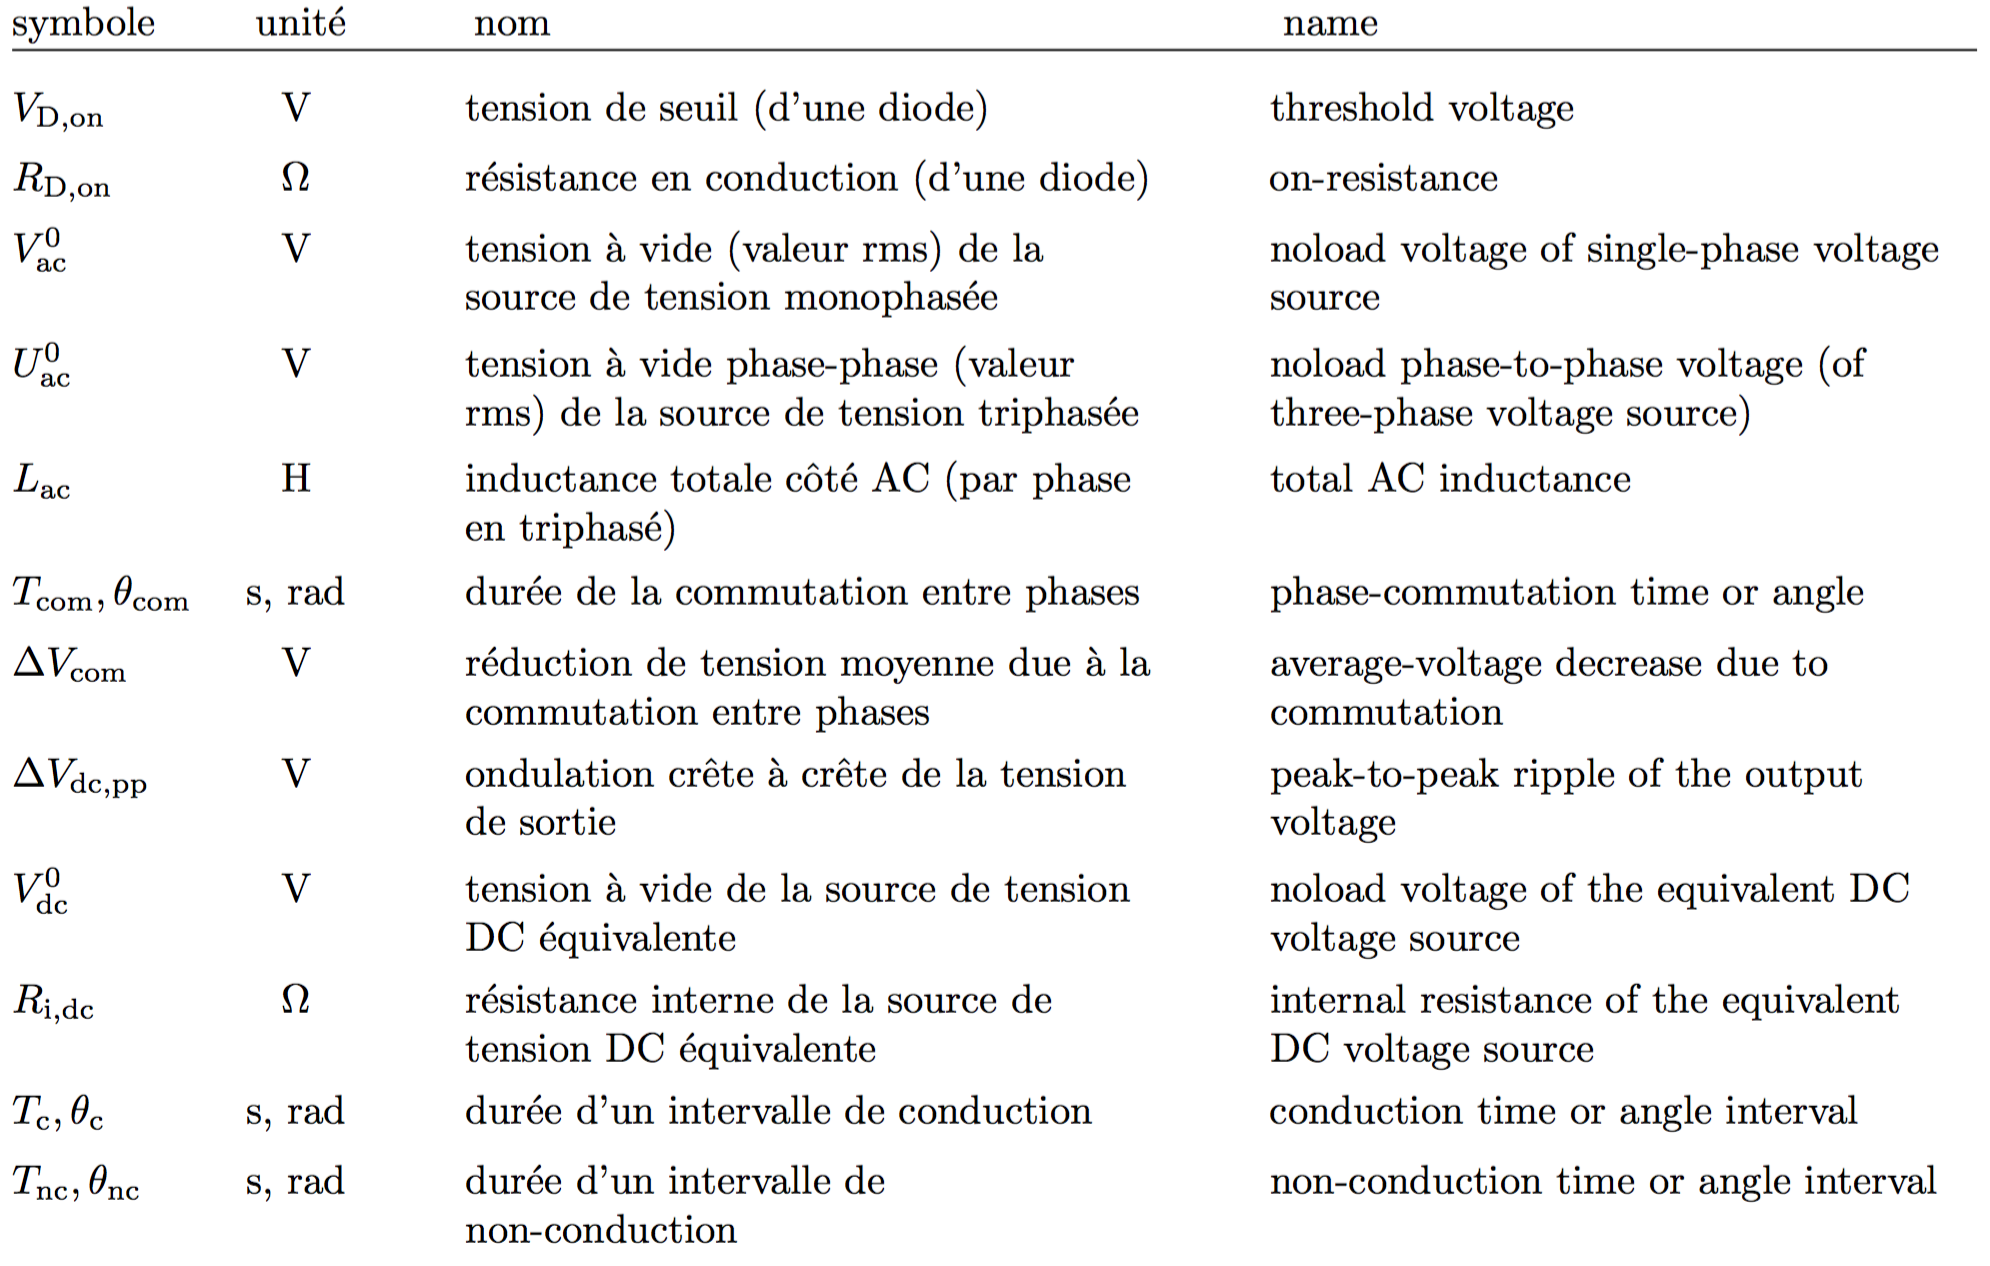
\includegraphics[scale=0.45]{ch2/1}
	\captionof{table}{Liste des symboles.}
	\end{center}
	\newpage
	
	\section{Caractéristique des diodes}
		La figure ci-dessous reprend la représentation réelle à idéalisée de la diode. Elle est \textbf{conductrice} ou passante pour $v_D=v_{AK}$ lorsque la tension entre l'anode $A$ et la cathode $K$ est positive. La tension dépend alors peu du courant $i_D$. 
		
		\begin{center}
		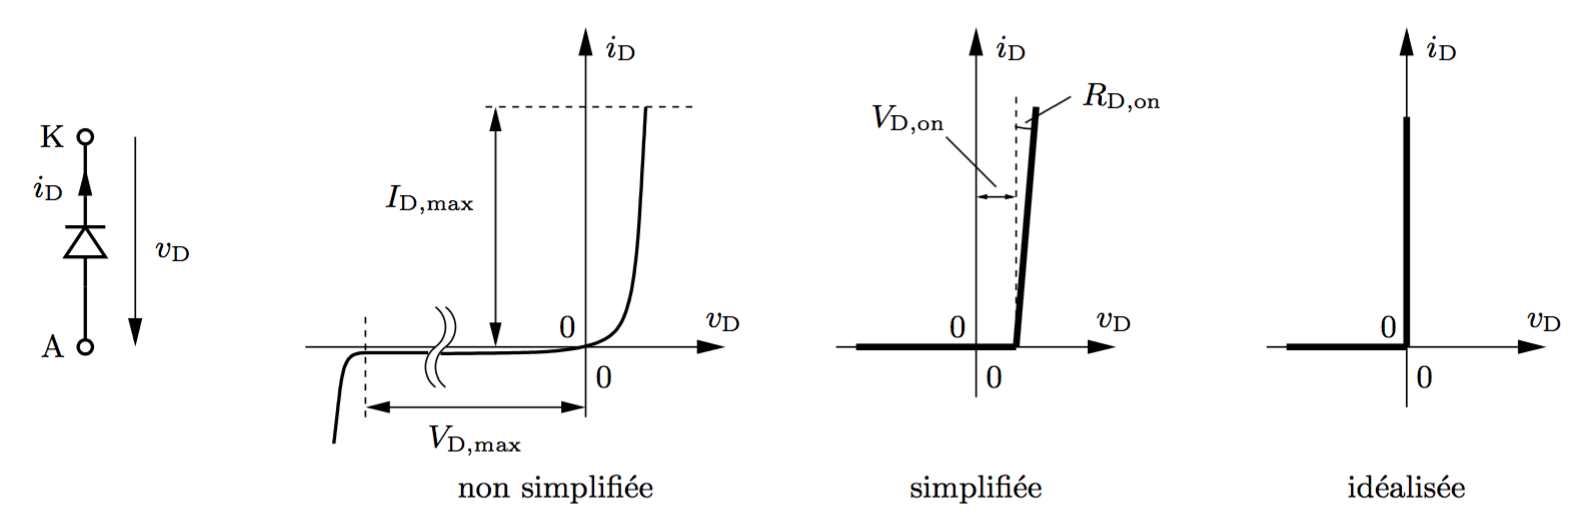
\includegraphics[scale=0.45]{ch2/2}
		\captionof{figure}{Modélisation d'une diode.}
		\end{center}			
		
		Le courant maximum qu'elle peut supporter, noté $i_{D,max}$ dépend de sa construction, sa taille et du radiateur, refroidisseur sur lequel elle est montée et peut atteindre plusieurs $kA$ pour celles sur le commerce. Pour les diodes de puissance, le transfert de chaleur vers le radiateur est essentiel. De plus elles ont une faible \textbf{inertie thermique} vu leur taille. Pour le modèle simplifié on a en conduction :
		\begin{equation}
			v_D = v_{D,on} + R_{D,on} i_D
		\end{equation}
		où $v_{D,on}$ est appelé \textbf{tension de seuil} et est de l'ordre du volt. Sauf pour les basses tensions (dizaine de volts ou moins), on négligera cette tension $v_D$ car elle influence peu les caractéristiques macroscopique des convertisseurs. On n'oubliera cependant pas qu'il existe une \textbf{perte de conduction} instantanée $P_D(t) = v_D(t)i_D(t)$. \\
	
		Pour ce qui est de l'état \textbf{bloquant} ou \textbf{bloqué}, il se manifeste lorsque $v_D < 0$ et $i_D$ sera négatif mais négligeable. La tension inverse maximum qu'on peut appliquer est noté $v_{D,max}$ et vaut plusieurs $kV$. Les diodes de puissance sont utilisées à des faibles \textbf{fréquences de commutation} (50 ou 60 $Hz$).
	
	\section{Charge inductive générique et circuits redresseurs élémentaires à une ou deux diodes}
		\subsection{Charge RLE générique}
			Pour l'étude des circuits, on considèrera une charge inductive générique RLE avec une résistance $R_{dc}$, une inductance $L_{dc}$ et une source de tension continue $E_{dc}$. Ces paramètres sont supposés constant c'est à dire que leur variation sur un cycle d'alimentation AC est négligeable. Ceci représente par exemple le circuit d'induit d'une MCC ($E_{dc}\neq 0$) ou son circuit d'excitation ($E_{dc}=0$). L'équation différentielle pour la tension aux bornes de la charge est :
			\begin{equation}
				v_{dc} = E_{dc} + R_{dc}i_{dc} + L_{dc}\frac{di_{dc}}{dt}.
			\end{equation}
			En régime établi et en introduisant la \textbf{tension moyenne} $V_{dc}$ et le \textbf{courant moyen} $I_{dc}$, on a :
			
			\begin{equation}
				V_{dc} = E_{dc} + R_{dc} I_{dc}.
			\end{equation}
			La charge étant alimenté par un redresseur à diode, $i_{dc}$ et $I_{dc}$ ne peuvent pas être négatifs et si $E_{dc}$ est trop élevé, le courant est nul. On a :
			\begin{equation}
				I_{dc} = max\left(\frac{V_{dc} - E_{dc}}{R_{dc}}\right).
			\end{equation}
			
			L'inductance de la charge tend à lisser le courant. C'est d'autant plus le cas que la constante de temps $\tau = L_{dc}/R_{dc}$ est grand par rapport à $T=1/f$ du réseau. Pour les ponts monophasé ou triphasé c'est l'intervalle de temps $T/2$ ou $T/6$ qui importe. Dans le cas d'une MCC, les ondulations de la tension implique une ondulation du courant et donc une ondulation du \textbf{couple électromagnétique}, ce qui est dérangeant. On peut donc adjoindre une inductance extérieur si c'est insuffisant, au détriment de performance dynamique réduits en cas de commande de couple, vitesse ou de position de l'entraînement électrique. 
			
		\subsection{Circuits redresseurs élémentaires avec une diode et une charge R, ER ou EL}
			\subsubsection{Avec charge R}
				La figure ci-dessous représente un circuit avec une source de tension AC de fréquence $f$ idéale raccordée à une diode idéale et une résistance avec $R_{dc}$ constante. Dans ce cas, $i_{ac}(t)=i_{dc}(t)$ à tout instant. La diode n'est passante que lorsque $v_{ac}(t)>0$, avec $v_{dc}(t)=v_{ac}(t)$ et $i_{dc}=v_{ac}(t)/R_{dc}$. La diode est bloquante lorsque $v_D=v_{ac}<0$, avec $v_{dc}=0=i_{dc}$.
				
				\begin{center}
					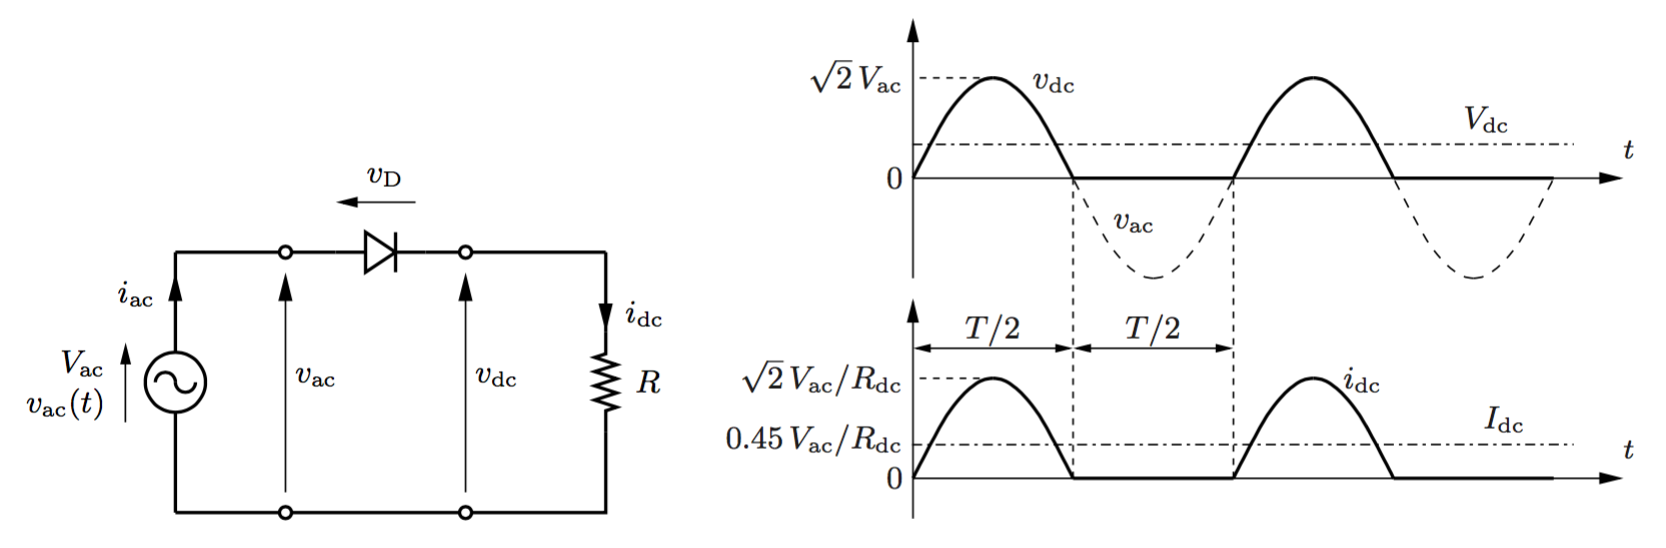
\includegraphics[scale=0.45]{ch2/3}
					\captionof{figure}{Montage redresseur élémentaire avec une diode et une résistance.}
				\end{center}
				
				On obtient la valeur moyenne de la tension en intégrant sur une demi-période de conduction :
				\begin{equation}
					V_{dc} = \frac{1}{2\pi} \int _0^\pi \sqrt{2}V_{ac}\sin (\omega t) \, d\omega t = \underbrace{\frac{\sqrt{2}}{\pi}}_{0.450} V_{ac}.
				\end{equation}
				